% journal_forward_density.tex
% A forward-looking density from one day of option quotes.
% Template/theme copied from journal_dec10_onward.tex (NTU Beamer); NEW FILE, that deck
% is not modified.
% Figures: figures/forward_density/*.pdf, built by
%   nn_boundary_deficit_results/forward_test/pub_compute.py  then
%   pub_evolution.py / pub_extraction.py / pub_realised.py / pub_consistency.py
%   Figure stems match the deck's figure numbers: fig1_* is captioned Figure 1.
% Numbers: figures/forward_density/fd_numbers.tex, built by pub_captions.py.
%          Every quantity cited below resolves through one of those macros, so the text
%          cannot drift away from the figures.
% Build: cd presentation && pdflatex journal_forward_density.tex   (twice)
\documentclass[aspectratio=169,11pt]{beamer}

\usetheme{default}
\setbeamertemplate{navigation symbols}{}
\setbeamertemplate{footline}[frame number]

\usepackage{booktabs}
\usepackage{amsmath,amssymb,amsfonts}
\usepackage{mathtools}
\usepackage{bm}
\usepackage{tikz}
\usetikzlibrary{shapes,arrows,positioning,calc,arrows.meta}
\usepackage{xcolor}
\usepackage{graphicx}
\usepackage{hyperref}

\graphicspath{{figures/forward_density/}{figures/}}
% Auto-generated by pub_captions.py -- do not edit by hand.
% Every figure number cited in the deck resolves through one of these macros.
\newcommand{\FDdate}{7 August 2001}
\newcommand{\FDspot}{5,752.51}
\newcommand{\FDrate}{4\%}
\newcommand{\FDrawrows}{421}
\newcommand{\FDnquotes}{217}
\newcommand{\FDnmat}{5}
\newcommand{\FDtaulo}{0.123}
\newcommand{\FDtauhi}{0.871}
\newcommand{\FDtaulist}{0.123, 0.200, 0.373, 0.603, 0.871}
\newcommand{\FDKtrainlo}{3,600}
\newcommand{\FDKtrainhi}{10,000}
\newcommand{\FDKlo}{100}
\newcommand{\FDKhi}{15,000}
\newcommand{\FDhfd}{50}
\newcommand{\FDhstar}{50}
\newcommand{\FDslopeRound}{-1.97}
\newcommand{\FDslopeTrunc}{+1.90}
\newcommand{\FDsweepBest}{1.5\times 10^{-4}}
\newcommand{\FDworstScale}{2.2\times 10^{-3}}
\newcommand{\FDworstCoreMean}{3.8\times 10^{-3}}
\newcommand{\FDpeakOverEnv}{105}
\newcommand{\FDmassWorst}{0.9995}
\newcommand{\FDfwdErr}{0.027\%}
\newcommand{\FDnegPct}{7.2\%}
\newcommand{\FDminFpct}{0.19\%}
\newcommand{\FDwinStart}{2001-08-07}
\newcommand{\FDwinEnd}{2002-11-01}
\newcommand{\FDwinN}{316}
\newcommand{\FDbandwidth}{0.316}
\newcommand{\FDhisSkew}{-0.80}
\newcommand{\FDhisSkewLog}{-1.05}
\newcommand{\FDoursSkewLo}{-0.75}
\newcommand{\FDoursSkewHi}{-0.42}
\newcommand{\FDoursSkewLogLo}{-2.19}
\newcommand{\FDoursSkewLogHi}{-1.51}
\newcommand{\FDfairLevel}{0.05}
\newcommand{\FDfairLog}{2.61}
\newcommand{\FDfairRatio}{54}
\newcommand{\FDmassFair}{0.9995}
\newcommand{\FDmcPaths}{40,000}
\newcommand{\FDmcSteps}{871}
\newcommand{\FDksWorst}{0.0047}
\newcommand{\FDksBest}{0.0024}
\newcommand{\FDlOneWorst}{0.0161}
\newcommand{\FDivWorst}{2.05}
\newcommand{\FDivRest}{0.33}
\newcommand{\FDmartWorst}{0.022\%}
\newcommand{\FDsdGapShort}{2.5\%}
\newcommand{\FDdtClosed}{35\%}
\newcommand{\FDdtRefine}{8}
\newcommand{\FDoutBandWorst}{51\%}
\newcommand{\FDqNegLo}{6\%}
\newcommand{\FDqNegHi}{25\%}
\newcommand{\FDqRatioLo}{2.7}
\newcommand{\FDqRatioHi}{6.9}
\newcommand{\FDqDKlo}{50}
\newcommand{\FDqDKhi}{400}
\newcommand{\FDqNegTot}{36}
\newcommand{\FDqIntTot}{207}
\newcommand{\FDnTauDense}{33}


\definecolor{ntunavy}{RGB}{0,32,91}
\definecolor{ntudarkblue}{RGB}{0,20,60}
\definecolor{ntured}{RGB}{192,32,38}
\definecolor{ntugold}{RGB}{255,204,0}
\definecolor{ntulightblue}{RGB}{100,150,200}

\setbeamercolor{background canvas}{bg=ntunavy}
\setbeamercolor{normal text}{fg=white}
\setbeamercolor{frametitle}{fg=white}
\setbeamercolor{title}{fg=white}
\setbeamercolor{subtitle}{fg=ntugold}
\setbeamercolor{author}{fg=ntugold}
\setbeamercolor{institute}{fg=white}
\setbeamercolor{date}{fg=ntured}
\setbeamercolor{item}{fg=ntugold}
\setbeamercolor{structure}{fg=ntugold}
\setbeamercolor{block title}{fg=white,bg=ntured}
\setbeamercolor{block body}{fg=white,bg=ntunavy!70!black}

\setbeamerfont{title}{size=\Large,series=\bfseries}
\setbeamerfont{frametitle}{size=\large,series=\bfseries}
\setbeamertemplate{itemize item}{\scriptsize\raise1.5pt\hbox{\textbullet}}
\setbeamertemplate{itemize subitem}{\scriptsize\raise1.5pt\hbox{\textendash}}

\newcommand{\gold}[1]{{\color{ntugold}#1}}
\newcommand{\red}[1]{{\color{ntured}#1}}

% Figure captions: full sentences, below the figure, in the register of a paper.
% What is shown, then what to conclude, then the one caveat that matters.
% ONE scale for every figure, so all six stay at identical effective font size.
% 0.97 buys ~5pt of vertical room per slide; 7.0pt labels land at 6.8pt.
\newcommand{\figw}{0.965}

\newcommand{\figcap}[2]{%
  \par\vspace{0.15ex}%
  % \centering is still active from the figure; restore justified setting so the
  % caption reads as a paragraph of prose rather than a centred block.
  {\tiny\setlength{\baselineskip}{1.08\baselineskip}%
   \leftskip=0pt\rightskip=0pt\parfillskip=0pt plus 1fil\relax
   \textbf{\gold{#1}}\hspace{0.4em}#2\par}}

\setbeamertemplate{background}{
    \begin{tikzpicture}[remember picture,overlay]
        \shade[left color=ntunavy,right color=ntudarkblue,shading angle=-45]
            (current page.north west) rectangle (current page.south east);
        \fill[ntured]
            (current page.north west) --
            ([xshift=1.8cm]current page.north west) --
            ([yshift=-2.7cm]current page.north west) -- cycle;
        \fill[ntured!85!black]
            ([yshift=-2.2cm]current page.north west) --
            ([xshift=1.4cm,yshift=-2.2cm]current page.north west) --
            ([yshift=-4.0cm]current page.north west) -- cycle;
    \end{tikzpicture}
}

\defbeamertemplate*{title page}{ntu}[1][]
{
    \begin{tikzpicture}[remember picture,overlay]
        \shade[left color=ntunavy,right color=ntudarkblue!90!ntunavy,shading angle=-30]
            (current page.north west) rectangle (current page.south east);
        \fill[ntured]
            (current page.north west) --
            ([xshift=2.2cm]current page.north west) --
            ([yshift=-3.3cm]current page.north west) -- cycle;
        \IfFileExists{ntu_logo.jpg}{
            \node[anchor=north west] at ([xshift=0.5cm,yshift=-0.4cm]current page.north west) {
                
\includegraphics[height=1.2cm]{ntu_logo.jpg}
            };
        }{}
        \node[anchor=north west, text width=11cm, font=\fontsize{11}{13}\selectfont\bfseries]
            at ([xshift=2.8cm,yshift=-2.0cm]current page.north west) {
            \textcolor{ntugold}{Dupire PINN --- deep self-consistent local volatility}
        };
        \node[anchor=north west, text width=11cm]
            at ([xshift=2.8cm,yshift=-2.7cm]current page.north west) {
            {\fontsize{19}{23}\selectfont\bfseries\color{white}\inserttitle}
        };
        \node[anchor=north west, text width=11cm, font=\fontsize{12}{14}\selectfont\bfseries]
            at ([xshift=2.8cm,yshift=-5.2cm]current page.north west) {
            \textcolor{ntugold}{\insertsubtitle}
        };
        \node[anchor=north west, text width=11cm, font=\fontsize{8}{10}\selectfont]
            at ([xshift=2.8cm,yshift=-6.1cm]current page.north west) {
            \textcolor{white}{\insertinstitute}
        };
        \node[anchor=north west, font=\fontsize{10}{12}\selectfont\bfseries]
            at ([xshift=2.8cm,yshift=-7.1cm]current page.north west) {
            \textcolor{ntured}{\insertdate}
        };
    \end{tikzpicture}
}

\setbeamertemplate{frametitle}{
    \vspace{0.3cm}
    \hspace{2.5cm}{\usebeamerfont{frametitle}\insertframetitle}
    \vspace{0.1cm}
}

\title{A forward-looking density\\from one day of option quotes}
\subtitle{Wang Z., Shaa A., Privault N., Guet C.}
\author{Ameir Shaa}
\date{\FDdate\ DAX --- \FDnquotes\ call quotes, \FDnmat\ maturities}
\institute{One calibration, no historical prices, no forecasting model}

\begin{document}
\maketitle

% ============================================================
% 1. The question
% ============================================================
\begin{frame}{The question}
  \small
  \begin{itemize}
    \item From a \gold{single day} of the DAX option market --- \FDdate, \FDnquotes\ active
          call quotes across \FDnmat\ maturities ($\tau=\FDtaulist$ yr), spot $S_0=\FDspot$
          --- recover the full \gold{probability density of the index at any future date}.
    \item No historical prices, no time-series model, no forecast. The only inputs are
          today's quotes and the requirement that the surface admit \gold{no arbitrage}.
    \item The density follows from that requirement alone: if $C(T,K)$ is arbitrage-free,
          then by Breeden--Litzenberger
          \[
            f_\tau(K) \;=\; e^{r\tau}\,\frac{\partial^2 C}{\partial K^2}(\tau,K)
          \]
          is the risk-neutral density of $S_\tau$ --- for \gold{every} $\tau$ the surface is
          defined at, not only the \FDnmat\ that happened to be quoted.
    \item \red{Three things must then be shown:} the second derivative is extracted
          correctly; the density is consistent with the model's own dynamics; and it stands
          up against what the index actually did.
  \end{itemize}
\end{frame}

% ============================================================
% 2. The mechanism
% ============================================================
\begin{frame}{The mechanism, in one slide}
  \small
  \begin{enumerate}
    \item \gold{Calibrate.} A network carries the normalised call price
          $\tilde\varphi(\tilde t,\tilde k)$ through the \gold{$\exp_k$ ansatz}
          \[
            \tilde\varphi=\exp\!\big(-\tilde k\,\mathrm{softplus}(a+\tilde k H)\big),
            \qquad a=y+\log\!\big(1-e^{-y}\big),\quad y=K_{\max}/S_0,
          \]
          $H$ the raw output. This makes $C(T,0)=S_0$ and unit mass hold \gold{by
          construction}, not as a fitted property --- the boundary is not something the
          optimiser can trade away.
    \item \gold{Close the loop.} Training is self-consistent: the same network supplies the
          Dupire local volatility
          $\sigma^2_{\mathrm{loc}}=2(\partial_TC+rK\partial_KC)/(K^2\partial^2_KC)$, and the
          price surface must satisfy the Dupire PDE it implies.
    \item \gold{Differentiate.} $\partial^2C/\partial K^2$ comes from nested automatic
          differentiation of the calibrated surface --- analytic in the network, evaluated
          at any $(\tau,K)$, with no interpolation between quoted expiries.
  \end{enumerate}
  \vspace{0.4ex}
  {\scriptsize Rate $r=\FDrate$; $K_{\max}$, $T_{\max}$ derived from the quotes, not set by hand.}
\end{frame}

% ============================================================
% 3. HERO
% ============================================================
\begin{frame}{One calibration $\rightarrow$ a density at every horizon}
  \centering
  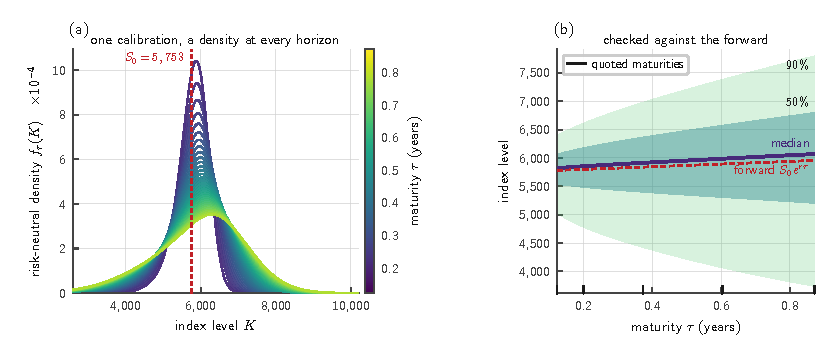
\includegraphics[width=\figw\linewidth]{fig1_evolution.pdf}
  \figcap{Figure 1.}{The risk-neutral density of the DAX implied by the \FDdate\
    calibration, shown (a) at \FDnTauDense\ maturities spanning the quoted range
    $\tau\in[\FDtaulo,\FDtauhi]$ yr, coloured by $\tau$, and (b) as the corresponding
    quantile fan against the forward $S_0e^{r\tau}$. The intermediate curves are not
    interpolated between fitted densities: each is read directly off the one calibrated
    surface, which is what makes a forward-looking distribution available at horizons that
    were never quoted. The distribution widens with $\tau$ and carries a heavier left tail
    than right --- the equity-index skew, recovered without being imposed.
    \red{Caveat:} the axis stops at the longest quoted expiry; nothing is extrapolated in
    $\tau$.}
\end{frame}

% ============================================================
% 3b. Why the quotes cannot simply be differenced
% ============================================================
\begin{frame}{Why not just difference the quotes?}
  \centering
  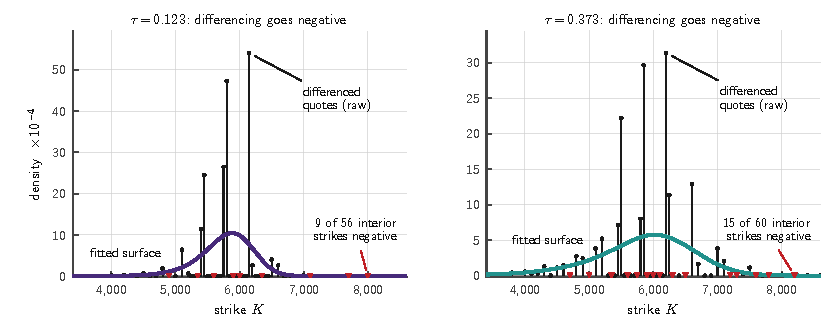
\includegraphics[width=\figw\linewidth]{fig2_quotes.pdf}
  \figcap{Figure 2.}{Breeden--Litzenberger applied \emph{directly} to the quoted call
    prices, with no surface in between: a three-point second difference on the quoted
    strike ladder (stems), against the density from the fitted surface (curve), at the two
    maturities with the most quotes. The ladder is spaced $\FDqDKlo$--$\FDqDKhi$ index
    points and the prices are rounded to the nearest $0.01$, so the second difference is
    dominated by where the rounding happens to put a kink: it spikes to
    $\FDqRatioLo$--$\FDqRatioHi\times$ the true peak, collapses to zero between spikes, and
    goes \red{negative} at $\FDqNegTot$ of $\FDqIntTot$ interior strikes
    ($\FDqNegLo$--$\FDqNegHi$ per maturity) --- a negative probability density. This is why
    a smooth arbitrage-free surface must be fitted first, and why the finite-difference
    check on the next slide is applied to that surface rather than to these prices.}
\end{frame}

% ============================================================
% 4. Extraction correctness
% ============================================================
\begin{frame}{Is the second derivative right?}
  \centering
  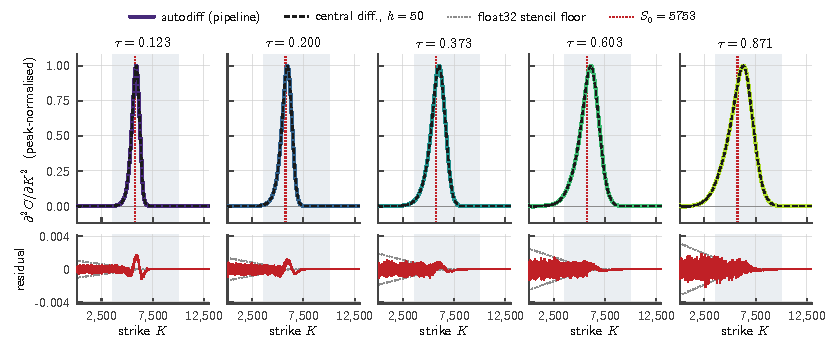
\includegraphics[width=\figw\linewidth]{fig3_extraction.pdf}
  \figcap{Figure 3.}{$\partial^2C/\partial K^2$ at each quoted maturity, read two
    independent ways, \gold{both applied to the fitted surface, not to the quoted prices}:
    the pipeline's nested automatic differentiation (colour) and a three-point central
    difference of the network's own call output at $K\pm\FDhfd$ (black dashed), each
    normalised by its own peak; the strip below shows the residual against the float32 stencil floor
    $4\varepsilon_{32}|C|/h^{2}$ (dotted). The two agree to $\FDworstScale$ of peak at
    worst, and away from the money the residual \emph{is} that floor --- no numerical
    headroom remains. The excursion at the money exceeds it by $\FDpeakOverEnv\times$
    and is genuine $h^{2}C''''/12$ truncation.
    \red{Caveat:} both routes read the same weights, so this tests the extraction, not the
    calibration; outside the shaded trained range both extrapolate.}
\end{frame}

% ============================================================
% 5. Step-size sweep
% ============================================================
\begin{frame}{The step size is chosen, not guessed}
  \centering
  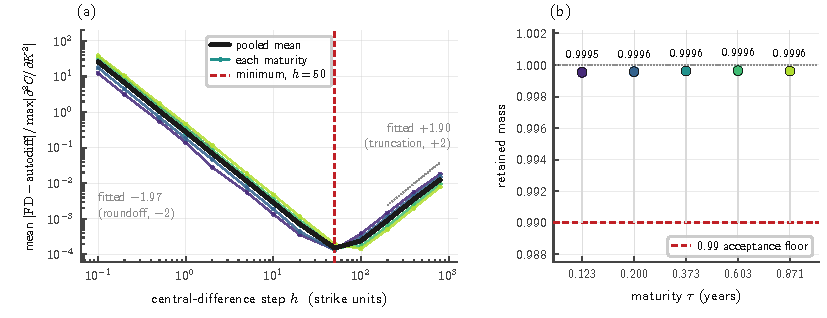
\includegraphics[width=\figw\linewidth]{fig4_stepsize.pdf}
  \figcap{Figure 4.}{(a) Mean disagreement between the finite-difference and automatic
    derivatives against the step $h$, per maturity and pooled. The curve is the classical
    U: the left branch has fitted log--log slope $\FDslopeRound$ against the $-2$ predicted
    by float32 round-off, the right branch $\FDslopeTrunc$ against the $+2$ predicted by
    $h^{2}$ truncation. Recovering both exponents from a trained network is what licenses
    reading the minimum at $h=\FDhstar$ as numerically optimal rather than tuned, and
    confirms the residual in Figure 3 is numerical, not structural. (b) Mass retained on
    $K\in[\FDKlo,\FDKhi]$, worst $\FDmassWorst$; the density mean reproduces the forward to
    $\FDfwdErr$. \red{Caveat:} the density is mildly negative on up to $\FDnegPct$ of grid
    points, all in the extrapolated tail outside the quoted strikes (worst excursion
    $\FDminFpct$ of peak) --- a convexity violation where there are no quotes.}
\end{frame}

% ============================================================
% 6. Against the realised path
% ============================================================
\begin{frame}{Against what the index actually did}
  \centering
  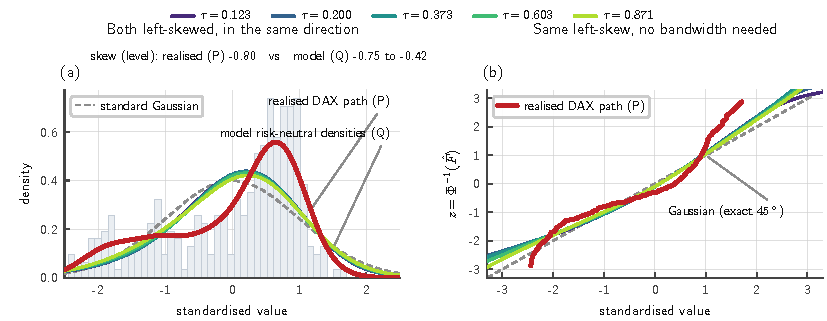
\includegraphics[width=\figw\linewidth]{fig5_realised.pdf}
  \figcap{Figure 5.}{The realised DAX path over the \FDwinN\ trading days from
    \FDwinStart\ to \FDwinEnd\ (red), discounted and standardised exactly as in
    N.~Privault's script, against the model's risk-neutral densities at the \FDnmat\ quoted
    maturities (colour): (a) densities at a common bandwidth $h=\FDbandwidth$ taken from
    the coarser series, each variance-corrected to s.d.\ 1 so widths are comparable;
    (b) the bandwidth-free normal-quantile view, where a Gaussian is exactly the
    $45^\circ$ line and curvature is skew. Both are clearly left-skewed and depart from the
    Gaussian in the same direction: realised skew $\FDhisSkew$ against $\FDoursSkewLo$ to
    $\FDoursSkewHi$. \red{This compares a risk-neutral
    ($\mathbb{Q}$) density against one realised path ($\mathbb{P}$)} --- different objects
    under different measures, $n=1$ on the $\mathbb{P}$ side, no change of measure applied
    --- so shape agreement is \emph{suggestive, not a formal test}. Second caveat: the same
    comparison in log space is not usable, since moving the left grid edge between two
    windows that both retain $\ge\FDmassFair$ of the mass shifts the log skew by
    $\FDfairLog$ but the level skew by only $\FDfairLevel$ ($\FDfairRatio\times$), so the
    log statistic reports where the grid was cut.}
\end{frame}

% ============================================================
% 7. Self-consistency
% ============================================================
\begin{frame}{Two independent routes to the same density}
  \centering
  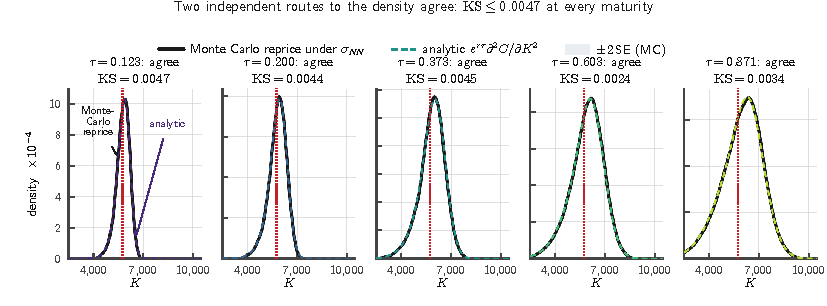
\includegraphics[width=\figw\linewidth]{fig6_selfconsistency.pdf}
  \figcap{Figure 6.}{The analytic density $e^{r\tau}\partial^2C/\partial K^2$ (dashed)
    against a Monte Carlo reprice of the \emph{same} surface under its own local volatility
    $\sigma_{NN}$ (black; $\FDmcPaths$ antithetic paths, $\FDmcSteps$ Euler steps), with the
    $\pm2$ MC standard-error band shaded. The two are obtained by genuinely different
    operations --- one differentiates the price surface twice in strike, the other simulates
    the SDE that surface implies and never sees the prices --- so agreement is an
    internal-consistency check, not a restatement. They agree to a Kolmogorov--Smirnov
    distance of $\FDksWorst$ at worst across all \FDnmat\ maturities, and the simulated
    forward matches $S_0e^{r\tau}$ to $\FDmartWorst$. \red{Caveat:} at the shortest maturity
    the analytic density is $\FDsdGapShort$ wider than the reprice, and refining the Euler
    step $\FDdtRefine\times$ closes only $\FDdtClosed$ of that gap, so part is time
    discretisation and part a real disagreement at short $\tau$.}
\end{frame}

% ============================================================
% 8. Closing
% ============================================================
\begin{frame}{The claim}
  \small
  \begin{itemize}
    \item From \gold{one day} of quoted option prices --- \FDnquotes\ calls on \FDdate\ ---
          we recover a \gold{full forward-looking probability density} of the DAX at any
          horizon out to the longest quoted expiry, using no historical prices and no
          forecasting model.
    \item It follows from no-arbitrage structure alone, via a calibrated Dupire surface
          whose boundary behaviour is built into the ansatz rather than fitted.
    \item It survives the checks that matter: extraction correct to $\FDworstScale$ of
          peak, with both theoretical error exponents recovered ($\FDslopeRound$,
          $\FDslopeTrunc$); self-consistent with its own dynamics to
          $\mathrm{KS}=\FDksWorst$; and its shape matches what the index did, in the one
          sense a single realised path can support.
    \item \red{What it is not:} a $\mathbb{P}$-measure forecast. It is the market's
          risk-neutral view on \FDdate\ --- exactly what is wanted for pricing and hedging,
          and what must be adjusted for a risk premium before being read as a prediction.
  \end{itemize}
\end{frame}

% ============================================================
% Appendix
% ============================================================
\begin{frame}{Appendix --- where the two densities differ}
  \centering
  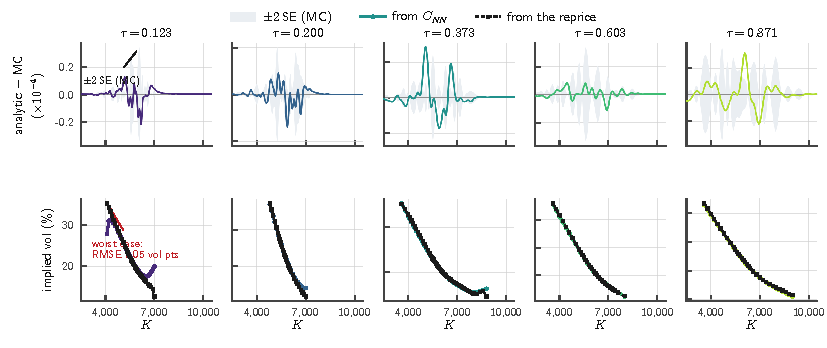
\includegraphics[width=\figw\linewidth]{figA1_residual.pdf}
  \figcap{Figure A1.}{Companion to Figure 6. Top: the analytic-minus-reprice density
    residual against the $\pm2$ MC standard-error band. Bottom: implied volatility on the
    quoted strikes, from the network's call prices and from the reprice. The residual is
    structured rather than noisy --- up to $\FDoutBandWorst$ of the grid lies outside twice
    the MC error at the shortest maturity --- but small in the terms that matter for
    pricing: the implied-volatility disagreement is $\FDivWorst$ vol points at the shortest
    maturity and at most $\FDivRest$ at every other one. The shortest maturity is where the
    Euler discretisation is coarsest relative to $\tau$, consistent with the $\mathrm{d}t$
    refinement reported in Figure 6.}
\end{frame}

\end{document}
